\documentclass{beamer}
\usepackage[british]{babel}
\usepackage[utf8]{inputenc} % This package will support Turkish chars

% Packages
\usepackage{hyperref}
\usepackage{stmaryrd}
\usepackage{color}
\usepackage{amsmath,amssymb}
\usepackage{graphicx}
\usepackage{fancyhdr}
\usepackage{ragged2e}
\usepackage{adjustbox}




% vertical separator macro
\newcommand{\vsep}{
  \column{0.0\textwidth}
    
\begin{tikzpicture}
      \draw[very thick,black!10] (0,0) -- (0,7.3);
    \end{tikzpicture}
}

% Beamer theme
\usetheme{Bilkent}
\usefonttheme[onlysmall]{structurebold}
\mode<presentation>
\setbeamercovered{transparent=10}

% align spacing
\setlength{\jot}{0pt}


% Intro info
\title{Investigating the Validity of Ground Truth in Code Reviewer Recommendation Studies }
\author[ESEM 2019]{
 \textbf{Emre Doğan}, Eray Tüzün, K. Ayberk Tecimer, H. Altay Güvenir}
\institute{MSc Student \newline Computer Engineering Department \newline Bilkent University \newline Ankara, TURKEY}
\date
    {\small\textit{{ESEM 2019}}\newline
    %Porto de Galinhas, Brazil \\
    \today
    }

\begin{document}

% Insert Titlepage before starting content.
\begin{frame}
  \titlepage
\end{frame}

% Insert table of contents if necessary
%\begin{frame}
%  \frametitle{Outline}
%
%  \small \tableofcontents
%\end{frame}


% Insert slides below.
\section{Introduction}

%\subsection{Code Review and Code Reviewer}

\begin{frame}{\large What is Code Review, Who is a Code Reviewer?}
    \textbf{Code Review:} A systematic examination of source code in order to highlight bugs and enhance the code quality.
    \pause
  \newline \newline
  \textbf{Code Reviewer:} The developer performing a code review who ensures the quality of the code.
  \pause
  \visible<3>{
  \vspace{-0.4cm}
  \begin{figure}
    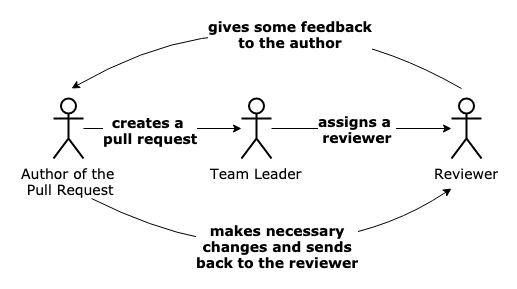
\includegraphics[height=0.5\textheight]{img/normal_review.png}
    \end{figure}
    \vspace{-0.7cm}
    \centering\color[rgb]{0,0.325,0.627}\textbf{A typical code review scenario}
    }
    
  %\begin{itemize}
  %    \item Using math equations
  %    \item Referencing Tables and Figures, as well as citations \cite{buyukccakir2018novel}
  %\end{itemize}
  
\end{frame}

%\subsection{Code Reviewer Recommendation}

\begin{frame}
\frametitle{How to find an ideal code reviewer?}

    %\begin{block}{Fact:}
    %\begin{itemize}
    %\item Code reviewing is not the most fun activity for a developer.
    %\item But it is a crucial step of software quality assurance process.
    %\end{itemize}
    %\end{block}
    %\pause
    \begin{itemize}
    \item Code reviewer recommendation models/tools help us to choose ideal reviewers.
    \item These tools help software teams:
        \begin{itemize}
            \item to find reviewers who can find more(critical) bugs in the source code.
            \item to speed up the code review process.
        \end{itemize}
  \end{itemize}


\end{frame}




%\subsection{Reviewer Selection}
\section{Real Life vs Algorithms}
\begin{frame}
\frametitle{\large Reviewer Selection in Recommendation Models }

  \begin{figure}
    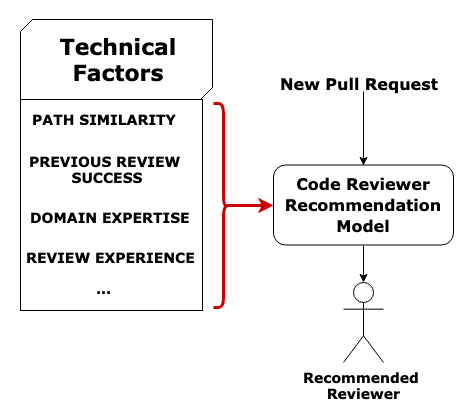
\includegraphics[scale=0.5]{img/algos.png}
    \end{figure}

\end{frame}

\begin{frame}
\frametitle{\large Reviewer Selection in Real Life }
  \begin{figure}
    \vspace{-0.3cm}
    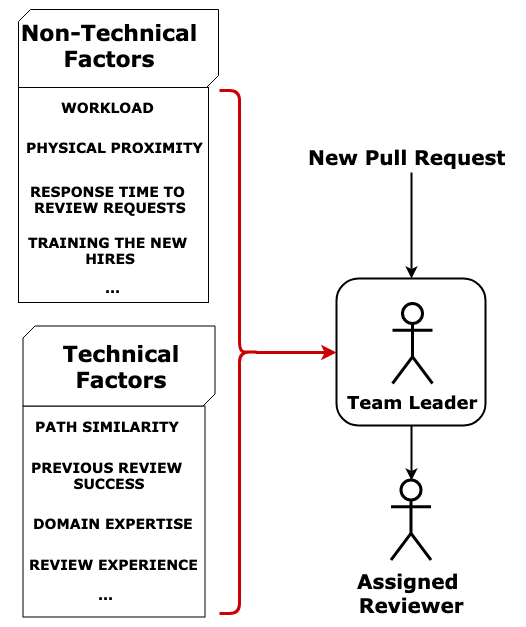
\includegraphics[height=1\textheight]{img/real-life.png}
    \end{figure}
\end{frame}

\begin{frame}
\frametitle{\large Comparison of Real Life and Algorithms}
  \begin{figure}
    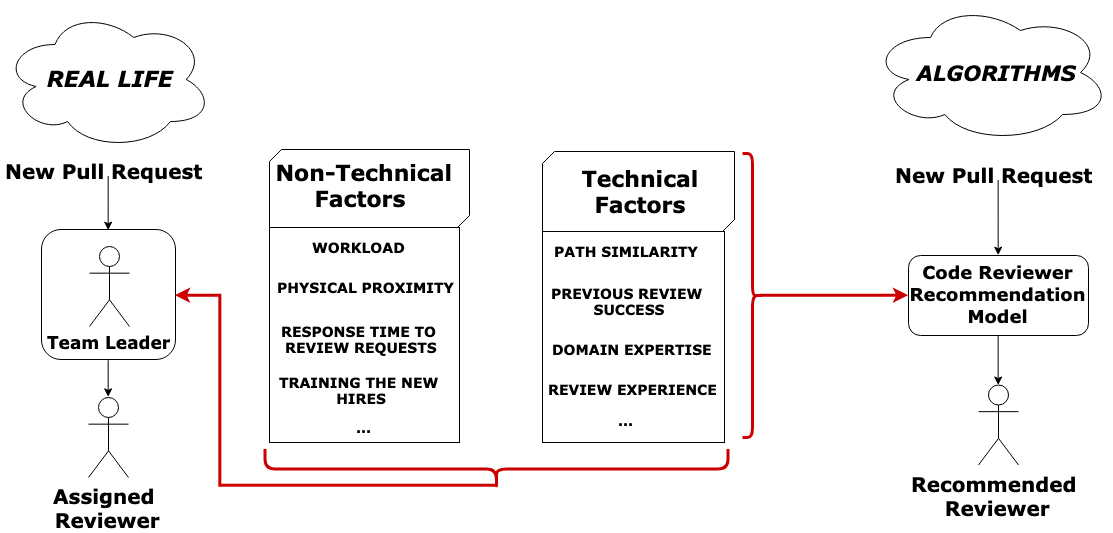
\includegraphics[width=0.83\textwidth]{img/comparison.png}
    \end{figure}
    \vspace{-0.24cm}
    \begin{alertblock}{Notice:}
        \begin{itemize}
        \item There exists a discrepancy between real life and algorithm based reviewer selection process.
        \item This discrepancy creates a \textbf{\textit{ground truth problem}} in code reviewer recommendation studies and datasets.
        \end{itemize}
    \end{alertblock}
\end{frame}

\section{Ground Truth}
\begin{frame}
\frametitle{\large Ground Truth}

    \begin{block}{Ground Truth:}
    \begin{itemize}
        \item Factual data that has been observed or measured.
        \item If data stands on some assumptions which is subject to opinion, then it cannot be \textbf{ground truth data}.
    \end{itemize}    
    \end{block}
    \pause
    \begin{block}{Ground Truth in Software Engineering:}
    \begin{itemize}
    \item The more human aspects involved, the more tendency to the ground truth problems.
    \item Many fields of empirical software engineering research suffer from the ground truth problem. (i.e. code reviewer recommendation, bug report assignee recommendation, etc.)   
    \end{itemize}    
    \end{block}    
\end{frame}


\begin{frame}
\frametitle{\large Ground Truth}

    \begin{block}{Ground Truth in Code Reviewer Recommendation Studies:}
    \begin{itemize}
        \item Recommendation models rely on the real-life assignments.
        \item These assignments are assumed to be ideal.
        \item Studies in real-life projects show that code reviewers are not usually assigned with the aim of finding the ideal one.
    \end{itemize}    
    \end{block}

\end{frame}
%\subsection{Ideal Reviewer}
\begin{frame}
\frametitle{\large Who is an ideal reviewer?}
 \hspace{5cm}{
 \begin{block}{Ideal Reviewer:}
        The theoretical best possible reviewer in the team that would improve or preferably perfect (such as pointing out all the defects) the pull request under review.
    \end{block}
    }
    \pause
    \begin{alertblock}{Warning:}
        \begin{itemize}
        \item Ideal reviewer is selected by considering \textbf{only technical factors}.
        \item I.e., If a developer is considered as the ideal reviewer for a pull request but is not available for a review at that moment, he/she is still the ideal reviewer.
        \end{itemize}
    \end{alertblock}
\end{frame}
\section{Example Scenario}
%\subsection{Problematical Reviewer Selection Scenario}
\begin{frame}
\frametitle{\large Problematical Reviewer Selection Scenario}
  \begin{figure}
    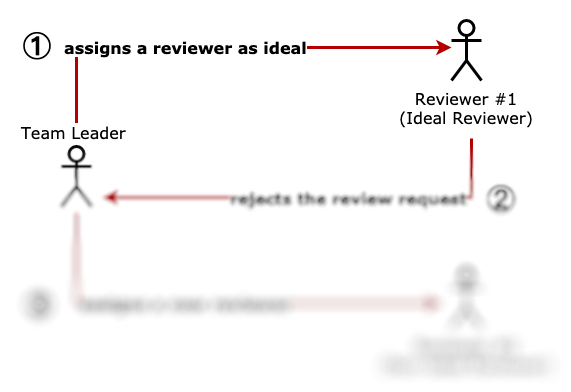
\includegraphics[height=0.8\textheight]{img/to_blur1.png}
    %\caption{lion!!}
    \end{figure}

\end{frame}

\begin{frame}
\frametitle{\large Problematical Reviewer Selection Scenario}
  \begin{figure}
    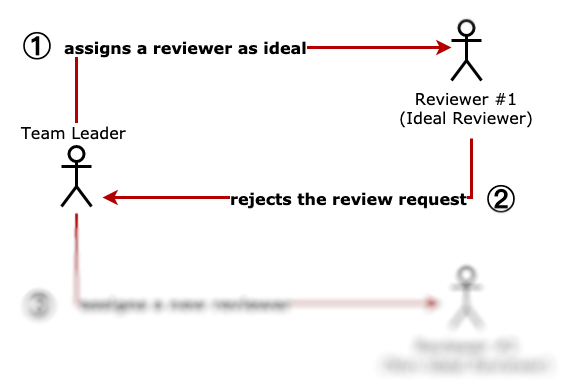
\includegraphics[height=0.8\textheight]{img/to_blur2.png}
    %\caption{lion!!}
    \end{figure}

\end{frame}
\begin{frame}
\frametitle{\large Problematical Reviewer Selection Scenario}
  \begin{figure}
    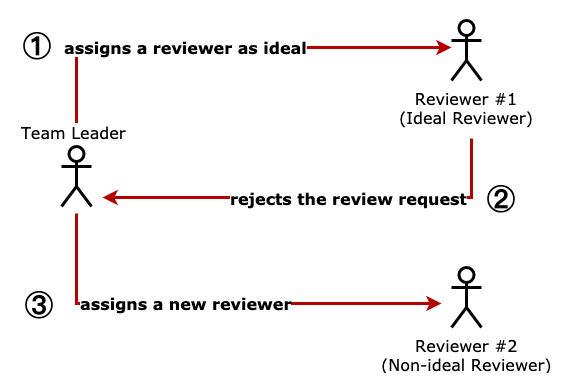
\includegraphics[height=0.8\textheight]{img/to_blur3.png}
    %\caption{lion!!}
    \end{figure}

\end{frame}


\iffalse
\subsection{Ideal Reviewer}
\begin{frame}
\frametitle{\large Who is an ideal reviewer?}
 \hspace{5cm}{
     \begin{block}{Ideal Reviewer:}
        The theoretical best possible reviewer in the team that would improve or preferably perfect (such as pointing out all the defects) the pull request under review.
    \end{block}
    }
    \pause
    \begin{alertblock}{Warning:}
        \begin{itemize}
        \item The selection of ideal reviewer is assumed to be completed by only technical factors.
        \item i.e. If a developer is considered as the ideal reviewer for a pull request but is not available for a review at that moment, he/she is still the ideal reviewer.
        \end{itemize}
    \end{alertblock}
\end{frame}
\fi

%%%%%%%%%%%%%%%%%%%%%%%%%%%%%%%%%%%%%%%%%%%
\section{Reasons of Non-Ideality}
\begin{frame}
\frametitle{\large What causes a non-ideal reviewer assignment?}
    \textbf{Availability Reasons:} \newline
    The ideal reviewer might be...
    \begin{itemize}
        \item  physically absent from work, so he/she cannot review the pull request. 
    \item  busy with some other tasks, so he/she declines to review the pull request.
    \item busy with some other tasks and is late to reply the review request.
    \end{itemize}
      \begin{figure}
      
\includegraphics[scale=0.1]{img/reviewer_available.jpg}
      \end{figure}

\end{frame}

%%%%%%%%%%%%%%%%%%%%%%%%%%%%%%%%%%%%%%%%%%%%%
\section{Quantitative Evidence}

\begin{frame}
\frametitle{\large Quantitative Evidence from Real Life }
        \begin{table}[]
        \centering
        \adjustbox{max height=\dimexpr\textheight-5.5cm\relax,
           max width=\textwidth}{
        \begin{tabular}{c|c|c|c}
        \textbf{Project Name} & \textbf{\begin{tabular}[c]{@{}c@{}}Total Number \\ of Pull Requests\end{tabular}} & \textbf{\begin{tabular}[c]{@{}c@{}}Number of PRs \\ with at least one \\ non-responsive reviewer\end{tabular}} & \textbf{\begin{tabular}[c]{@{}c@{}}The ratio of PRs \\ having at least one \\ non-responsive reviewer\end{tabular}} \\
        \hline
        Android & 36,771 & 24,367 & 66\% \\
        \hline
        LibreOffice & 18,716 & 3,039 & 16\% \\
        \hline
        Open Stack & 108,788 & 24,589 & 23\% \\
        \hline
        Qt & 65,815 & 30,630 & 47\% \\
        \hline
        TOTAL & 230,090 & 82,625 & 36\%
        \end{tabular}}
        \caption{An Analysis of Pull Request Reviews from 4 Large OSS Projects\footnote{\tiny S. Ruangwan, P. Thongtanunam, A. Ihara, and K. Matsumoto, “The impact of human factors on the participation decision of reviewers in modern code review,”\textit{ Empirical Software Engineering}, vol. 24, no. 2,pp. 973-1016, 2019. pp. 973–1016, 2019.}}
        \label{tab:my-table}
        \end{table}
        \begin{alertblock}{Notice}
        \large The results illustrate that 36\% of pull requests suffer from the \textit{availability reasons}. 
        \end{alertblock}
    \end{frame}

%
%\subsection{Cognitive Bias}
\begin{frame}
\frametitle{\large What causes a non-ideal reviewer assignment?}
     \begin{block}{Cognitive Bias:}
        A systematic pattern of deviation from norm or rationality in judgment.
    \end{block}
    \pause
     \begin{block}{Attribute Substitution:}
        {It occurs when an individual has to make \textbf{a computationally complex judgment}, and instead substitutes \textbf{a more easily calculated heuristic attribute}.}
    \end{block}
    \pause
    \begin{columns}
    \begin{column}{0.6\textwidth}
    The team leader prefers to assign...
      \begin{itemize}
    \item  a volunteer for the review.
    \item   a reviewer based on their work schedule.
    \item a new hire as a reviewer for educational purposes.
    \item a developer based on their relative response time to review requests.
    \end{itemize}
    \end{column}
    \begin{column}{0.4\textwidth}  %%<--- here
      \begin{figure}
      
\includegraphics[scale=0.2]{img/cog_bias.jpg}
      \end{figure}
\end{column}
\end{columns}


\end{frame}



    
%%%%%%%%%%%%%%%%%%%%%%%%%%%%%%%%%%%%%%%%%%%%%%%%%%%    
%%%%%%%%%%%%%%%%%%%%%%%%%%%%%%%%%%%%%%%%%%%%%%%%%%%
%%%%%%%%%%%%%%%%%%%%%%%%%%%%%%%%%%%%%%%%%%%%%%%%%%%
\iffalse
\section{Solution Alternatives}
    \begin{frame}{Solution Alternatives}
    We provide two possible solutions to establish ground truth data: \newline
    \begin{itemize}
        \item Setting up an Experiment in Real Life
        \item Forward-Looking Mining the Issue Repository
    \end{itemize}
    \end{frame}
    \fi


%%%%%%%%%%%%%%%%%%%%%%%%%%%%%%%%
%%%%%% implications%%%%%%%%%
\section{Conclusion}
\begin{frame}{Implications of This Study}
\begin{itemize}
    \item\large Previous reviewer recommendation studies and datasets should be reviewed in terms of the validity of the ground truth.
    \pause
    \item\large New recommendation models and datasets should be created by considering this validity problem.
    \pause
    \item\large A validated benchmark dataset for reviewer recommendation task should be created.  
\end{itemize}

\end{frame}
%%%%%%%%%%%%%%%%%%%%%%%%%%%%%%%%
%\section{Conclusion \& Future Work}
\begin{frame}{Conclusion}

\begin{itemize}
    
    \item\large The validation of real-life collected reviewer datasets are problematic.
    \pause
   \item\large The validation problem of these datasets affect the validity of recommendation models.    
    \iffalse
    \pause
    \item\large This problem is valid for other software engineering tasks such as bug report assignee recommendation.
    \fi

\end{itemize}
\end{frame}
\begin{frame}{Future Work}

\begin{itemize}
    \item Introducing quantitative evidence for cognitive bias.
    \pause
    \item Establishing ground truth data by alternative solutions.
    \pause
    \item Check our paper for solution proposals:
    \begin{itemize}
        \item Setting up an Experiment in Real Life
        \item Forward-Looking Mining the Issue Repository
    \end{itemize}
\end{itemize}
\end{frame}



\iffalse
\begin{frame}{Future Work}

\begin{itemize}
    \item Introducing quantitative evidence for cognitive bias.
    \pause
    \item Exploring alternative solutions for this problem.
\end{itemize}
\end{frame}

\begin{frame}{For the full-text PDF:}
\centering \Large https://bit.ly/2koV4Jk

\vskip 0.12in

\centering \Large or

\vskip 0.12in


\includegraphics[width=0.4\textwidth]{img/qr_code_researchgate.png}
\end{frame}
\fi

%%%%%
\begin{frame}{Thank you}

\begin{columns}
\begin{column}{0.5\textwidth}
\centering \normalsize Emre Doğan

\centering \small \textit{MSc Student}

\centering \small Computer Engineering Department

\centering \small Bilkent University 

\centering \small Ankara, Turkey

emre.dogan@bilkent.edu.tr
\end{column}
\begin{column}{0.5\textwidth}  %%<--- here
\centering \Large https://bit.ly/2koV4Jk

\vskip 0.12in

\newline

\vskip 0.12in


\includegraphics[width=0.4\textwidth]{img/qr_code_researchgate.png}
\end{column}
\end{columns}
\end{frame}

%%%%%

\iffalse
\begin{frame}{Any Questions}

\centering \normalsize Emre Doğan

\centering \small \textit{MSc Student}

\centering \small Computer Engineering Department

\centering \small Bilkent University 

\centering \small Ankara, Turkey

emre.dogan@bilkent.edu.tr
\end{frame}
\fi


\section{After the Presentation}
%%%%%%%%%%%%%%%%%%%%%%%%%%%%
\begin{frame}[noframenumbering]{Backup Slides}
\end{frame}

\begin{frame}[noframenumbering]{\large Possible Reviewer Assignment Scenarios}
      \begin{figure}
      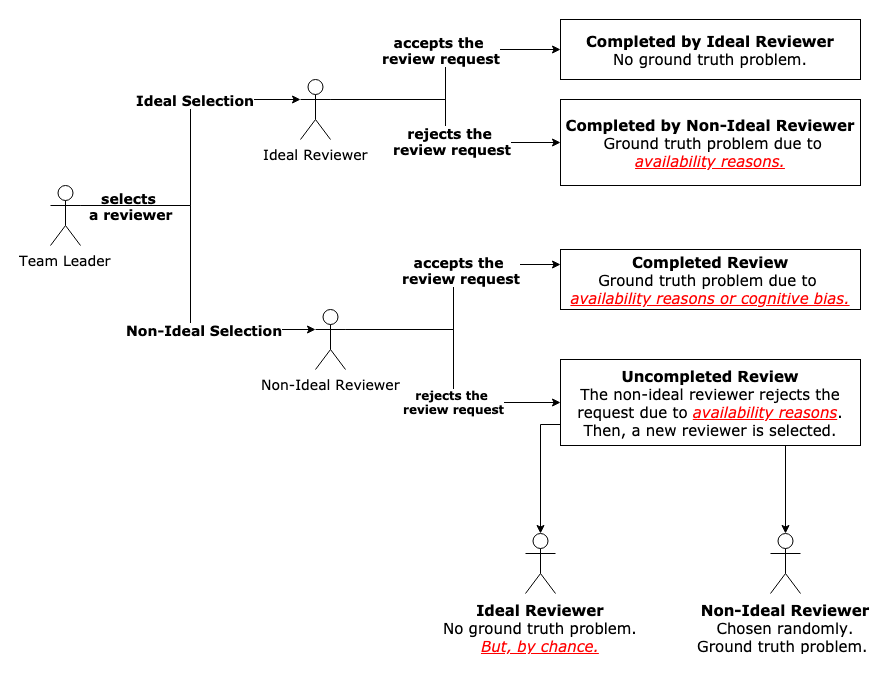
\includegraphics[width=0.8\textwidth]{img/scenarios_all.png}
      \end{figure}
\end{frame}
%%%%%%%%%%%%%%%%%%%%%%%%%%%%
\begin{frame}[noframenumbering]{\large Scenario 1}
      \begin{figure}
      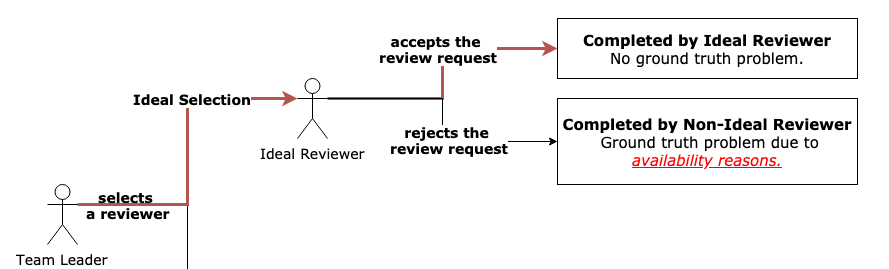
\includegraphics[width=1.05\textwidth]{img/scenarios_1.png}
      \end{figure}
\end{frame}
%%%%%%%%%%%%%%%%%%%%%%%%%%%%
\begin{frame}[noframenumbering]{\large Scenario 2}
      \begin{figure}
      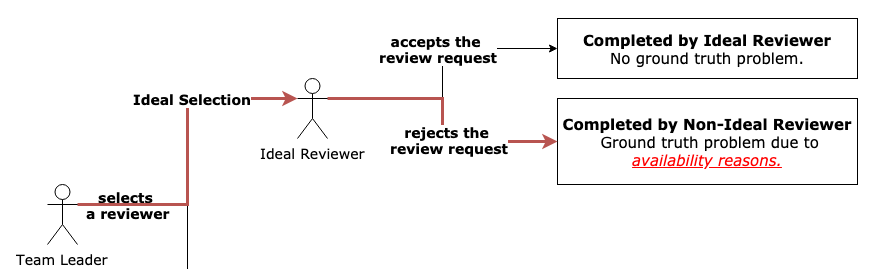
\includegraphics[width=1.05\textwidth]{img/scenarios_2.png}
      \end{figure}
\end{frame}
%%%%%%%%%%%%%%%%%%%%%%%%%%%%
\begin{frame}[noframenumbering]{\large Scenario 3}
      \begin{figure}
      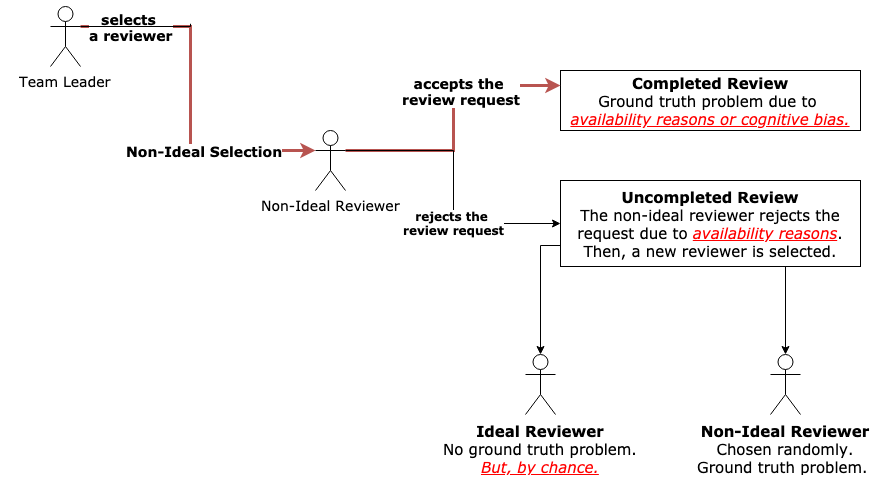
\includegraphics[width=1.05\textwidth]{img/scenarios_3.png}
      \end{figure}
\end{frame}
%%%%%%%%%%%%%%%%%%%%%%%%%%%%
\begin{frame}[noframenumbering]{\large Scenario 4}
      \begin{figure}
      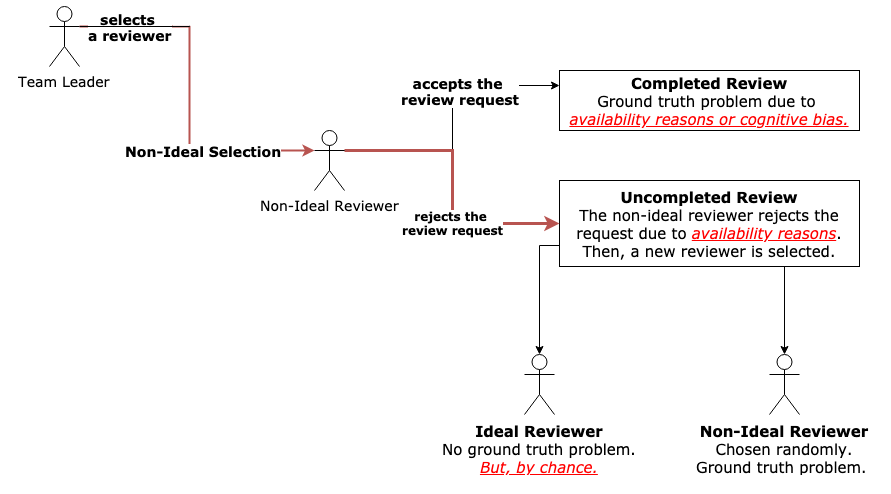
\includegraphics[width=1.05\textwidth]{img/scenarios_4.png}
      \end{figure}
\end{frame}
%%%%%%%%%%%%%%%%%%%%%%%%%%%%
\iffalse
\section{Quantitative Evidence}
\begin{frame}
\frametitle{\large Data, data, data...}
 \begin{columns}
    \begin{column}{0.37\textwidth}
    \begin{figure}
      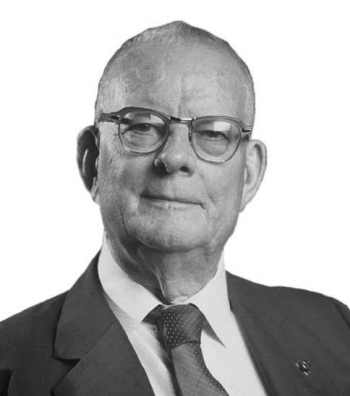
\includegraphics[width=\textwidth]{img/edward_deming.png}
     \end{figure}
     
    \end{column}
    \begin{column}{0.55\textwidth}  %%<--- here
    \hspace{-0.1cm}
    \centering\Large Without data, you're just another person with an opinion.\newline\newline
     \centering\small\textit{Dr. W. Edwards Deming}
\end{column}
\end{columns}
\end{frame}
\fi


    %%%%%%%%%%%%%%%%%%%%%%%%%%%%
    %%%%SOLUTION ALTERNATIVES%%%
    %%%%%%%%%%%%%%%%%%%%%%%%%%%%

    \begin{frame}[noframenumbering]{Solution Alternatives}
    I - Setting up an Experiment in Real Life\newline
    II - Forward-Looking Mining
    \end{frame}
    \begin{frame}[noframenumbering]{Solution I- Setting up an Experiment in Real Life}
        \centering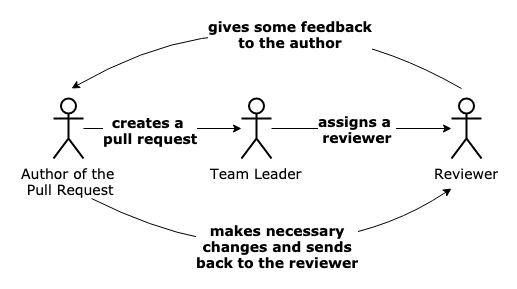
\includegraphics[width=0.85\textwidth]{img/normal_review.png} \newline
        \centering\color[rgb]{0,0.325,0.627}\textbf{A Typical Reviewer Assignment Scenario}
    \end{frame}

    \begin{frame}[noframenumbering]{What if...}
        ... we assign the same review to multiple reviewers simultaneously?
        \centering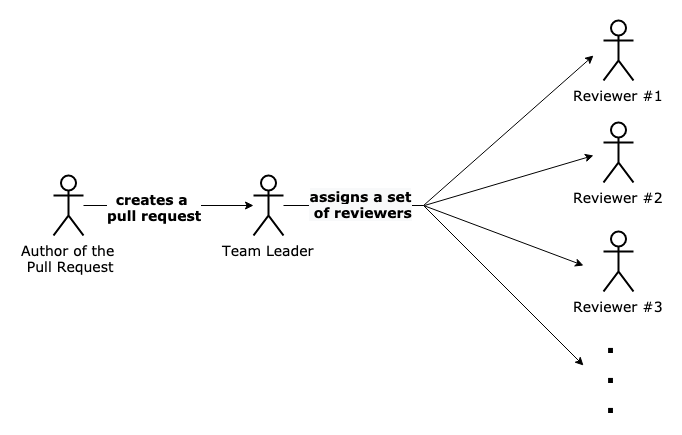
\includegraphics[width=0.9\textwidth]{img/multiple_review.png}
    \end{frame}


    \begin{frame}[noframenumbering]{Then, choose the best one}
        \centering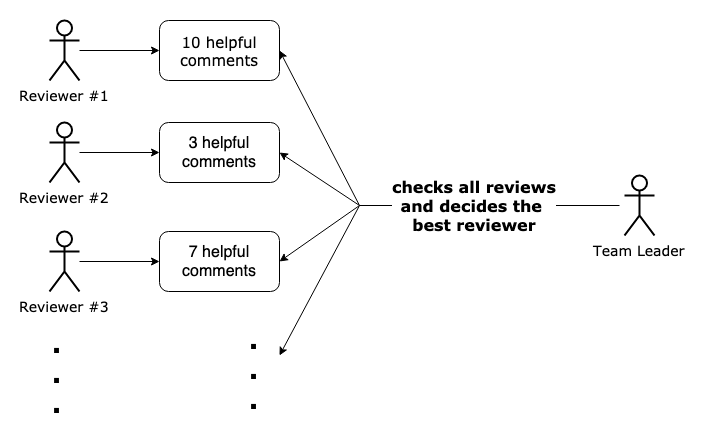
\includegraphics[width=0.9\textwidth]{img/multiple_review_2.png}
    \end{frame}

    \begin{frame}[noframenumbering]{Then, choose the best one}
        \centering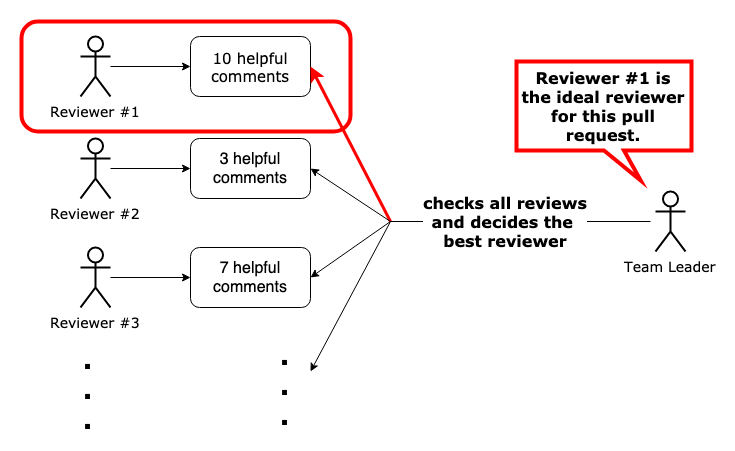
\includegraphics[width=0.9\textwidth]{img/multiple_review_3.png}
    \end{frame}
    
    \begin{frame}[noframenumbering]{What is wrong with this method?}
    \begin{alertblock}{Expensive!}
        Making multiple developers spend time on a single review task is impractical and expensive.
    \end{alertblock}
    \pause
    \begin{alertblock}{Hard to evaluate!}
        It is not a straightforward task for the team leader to check all reviews and choose the best one.
    \end{alertblock} 
    \end{frame}
    
    %%%%%%%%%%%%%%%%%%%%%%%%%%%%%%%%%%%%%%%%%%%%%%%%%%%%%%%%%%%%%%%%%%%%%%%%%%%%%%%%%%%%%%%%%%%%%%%%%%%%
    \begin{frame}[noframenumbering]{Solution II - Forward-Looking Mining}
        \begin{block}{Idea:}
        Reopened bugs might indicate a bad code review.
        \end{block}
        \pause
        \begin{exampleblock}{How?}
        Consider the following scenario.
        \end{exampleblock}
    \end{frame}
    
    \begin{frame}[noframenumbering]{Consider the following scenario:}
    \centering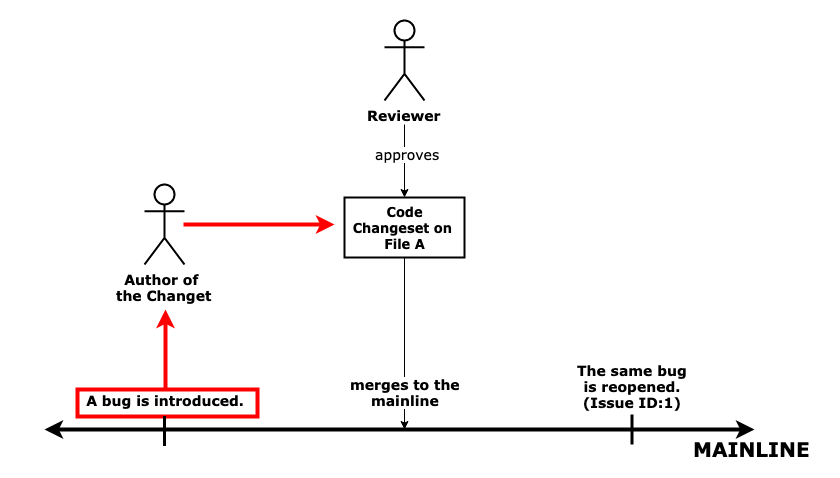
\includegraphics[width=0.9\textwidth]{img/future_mining_1.png}\newline\newline
    \caption{To fix a bug, a developer creates a pull request.}
    \end{frame}
    
    \begin{frame}[noframenumbering]{Consider the following scenario:}
    \centering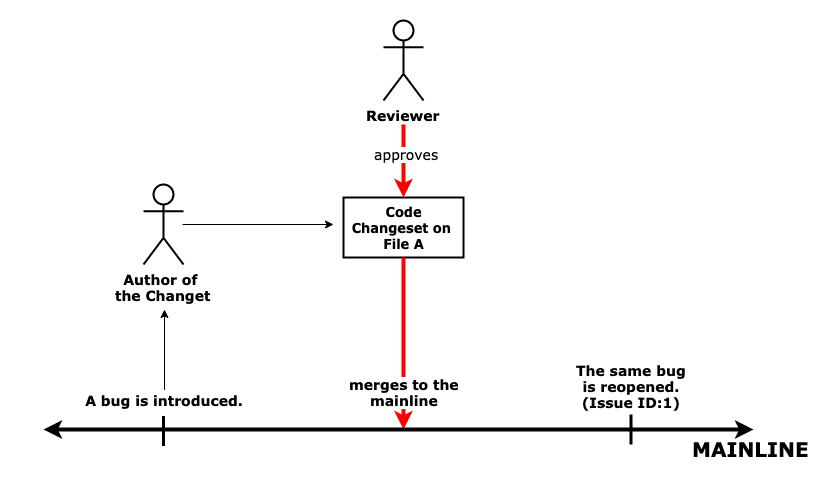
\includegraphics[width=0.9\textwidth]{img/future_mining_2.png}\newline\newline
    \caption{The assigned reviewer approves the pull request and the bug is closed.}
    \end{frame}  
    
    \begin{frame}[noframenumbering]{Consider the following scenario:}
    \centering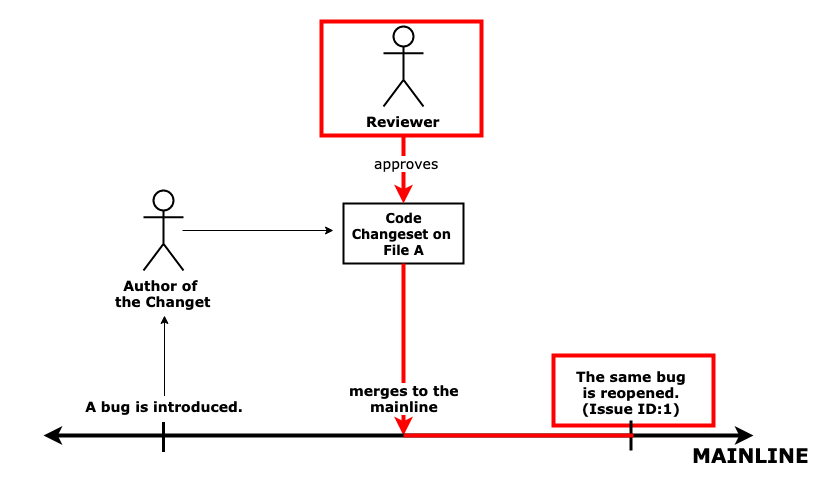
\includegraphics[width=0.9\textwidth]{img/future_mining_3.png}\newline
    \caption{If the same bug is reopened later, it is a potential indicator that the pull request is not conducted properly and the reviewer is not ideal.}
    \end{frame}

    \begin{frame}[noframenumbering]{Consider the following scenario:}
    \centering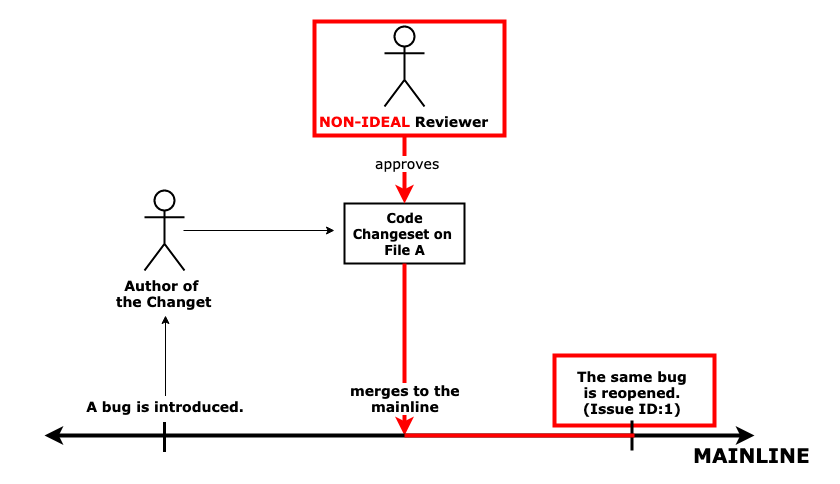
\includegraphics[width=0.9\textwidth]{img/future_mining_4.png}\newline
    \caption{Removing these instances from the dataset will increase the validity of ground truth.}
    \end{frame}

%\section{References}
%\begingroup
%\Tiny
%\begin{frame}[allowframebreaks]
%    \frametitle{References}
%    \bibliographystyle{apalike}
%    \bibliography{bibliography} 
%\end{frame}
%\endgroup
  %\cite{buyukccakir2018novel}

\end{document}
